\documentclass{beamer}
\usepackage[utf8]{inputenc}
\usepackage{graphicx}

% themes found here: https://latex-beamer.com/tutorials/beamer-themes/
\usetheme{PaloAlto}
\setbeamertemplate{footline}[frame number]

\title{Resilient Weather Kriging}

% TODO: add names
\author{
    Baxter, Hunter %\\
    % \and
}

\begin{document}
\maketitle

\section{Architecture}
\begin{frame}{Architecture}
% we should update this figure
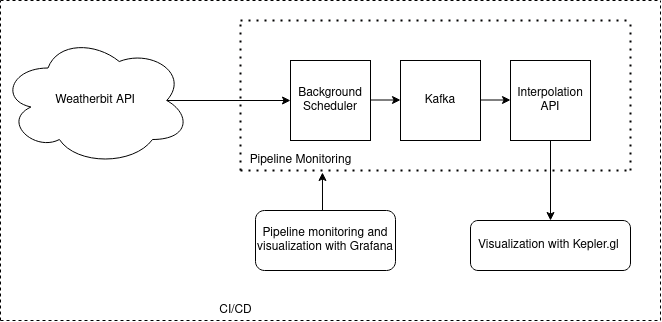
\includegraphics[width=\linewidth]{figures/architecture.png}
\end{frame}

\section{CI/CD}
\begin{frame}{CI/CD}
\begin{itemize}
    \item Minimimum viable product currently uses Github Actions
    \item end goal is to use jenkins
    % insert image of pipeline if we go with jenkins, otherwise this slide not be worth including
\end{itemize}
    
\end{frame}

\section{Data}
\begin{frame}{Data}
% basic information about weatherbit and why real time weather data matters (ex. road conditions, agriculture) 
\end{frame}

\section{Pipeline}
\begin{frame}{Pipeline}
\end{frame}

\section{Kriging}
\begin{frame}{Kriging}
% insert information about proposed kriging and why it is necessary
\end{frame}

\section{Front-End}
\begin{frame}{Front-End}
% insert kepler.gl front-end application information
\end{frame}

\end{document}